\documentclass{llncs}
\usepackage{enumerate,graphicx}
\usepackage{graphicx}
\usepackage{amsmath,amssymb}
\usepackage{algorithm,lipsum}
\usepackage[noend]{algpseudocode}
\usepackage{graphicx}
%\usepackage{titling}

%\newcommand{\subtitle1}[1]{%
%	\posttitle{%
%	\begin{center}\large#1\end{center}
%	\vskip0.5em}%
%}

\title{Safety Critical Systems Project Report \\ Predictive Maintenance in Vehicle Systems}
\author{Pushpita Sarkar(Matriculation No: 1384152)\and Nidhi Nayak (Matriculation No: 1404524)\and Deepak Kumar (Matriculation No: 1400489)\and Ashlesh Mithur (Matriculation No: 1386367)}
\institute{Frankfurt University of Applied Sciences}

% this is how you can define macros
\newcommand{\T}{\mathcal{T}}
\newcommand{\I}{\mathcal{I}}
\renewcommand{\L}{\mathcal{L}}

\begin{document}

\maketitle

%\begin{abstract}
%	\label{sec:abstract}
This document is a model and instructions for \LaTeX.
This and the IEEEtran.cls file define the components of your paper [title, text, heads, etc.]. *CRITICAL: Do Not Use Symbols, Special Characters, Footnotes, 
or Math in Paper Title or Abstract. Edited
%\end{abstract}


\section{Introduction}
\label{sec:introduction}
This document is a model and instructions for \LaTeX.
Please observe the conference page limits. Bla bla

\section{Process Model}
\label{sec:process-model}
Agile-Scrum software development:  Scrum is an agile methodology where products are developed iteratively. Planning, sprints, stand-ups, and retrospectives are integral parts of scrum methodology. In this model we are going to use Vmodel XT in combination with Agile scrum.

\section{Team Organization}
\label{sec:team-organization}
This document is a model and instructions for \LaTeX.
Please observe the conference page limits. Bla bla

\section{Task Distribution}
\label{sec:task-distribution}
Since we are following Agile-Scrum methodology, we will be having bi-weekly scrums wherein we will discuss updates related to the tasks assigned and blockers if any. Since we are a small team of 4 people, every member will contribute in all the phases of the project life-cycle.

\section{Requirement Management}
\label{sec:requirment-management}
\begin{itemize}
\item Read Literature.
\item Understand the real-world use-cases of predictive maintenance.
\end{itemize}

\section{Use Cases}
\label{sec:use-case}
\begin{itemize}
	 \item \textbf{Anti-lock Braking system and Traction Control Systems:} ABS components include: a wheel- speed sensor, a hydraulic modulator and an Electronic Control Unit (ECU) for signal processing and control and triggering of the signal lamp and of the actuators in the hydraulic modulator.
	 If any of these components malfunction and the user is not notified in time to take corrective steps, there can be grave danger to the driver’s, passengers’ and pedestrians’ lives.
	 
	 \item \textbf{Airbags:} There are a number of other reasons that may cause the airbags to fail.
	 \begin{enumerate}
	 	\item \textbf{Airbag backup battery} has already been depleted- Check for it have a threshold voltage that battery must have, and notify to users immediately.
	 	\item \textbf{Faulty Sensors:} Sensors may malfunction or be inadvertently tripped, which might fail to deploy during actual crash.
	 	\item \textbf{Soaked Airbag Module:} If your vehicle has been touched by water damage (maybe have a sensor to get the moisture level if it is regularly exposed and increasing moisture/water particles.
	 	\item \textbf{Damaged Airbag Clock Spring:} he airbag clock spring is there for the continuity between the electrical wiring of your vehicle and your driver-side airbag. The rotary electrical connector allows the steering wheel to turn while keeping a connection between the wheel’s airbag, horn, and the electrical system. So, if the clock spring isn’t working, then the airbag won’t deploy. The clock spring will coil in and out with every turn of your steering wheel so it is only normal that it will become worn out over time. The poor connection will give way for potential airbag failures 
	 \end{enumerate}
	 
	 \item \textbf{Seat belt system switch sensors:} Seat belts plays major role in safety for effective working of airbags.
	 
	 \item \textbf{Autonomous Emergency braking system }is a crucial part of the autonomous car. It one of the standard safety equipment of a self-driving car. This AEB works by scanning the distance of the road measuring the distance of the front road. And everything is controlled here by using sensors like ultrasonic sensors etc. If these sensors don’t work properly collision may occur. So, one of the approaches of our system to diagnose whether these sensors work properly, if not it will notify the user for maintenance.
	 
	 \item \textbf{Air pressure systems} also called as compressed air brake system, is a type of friction brake for vehicles in which compressed air pressing on a piston is used to apply the pressure to the brake pad or brake shoe needed to stop the vehicle. Air brakes are typically used in heavy trucks and buses. Typical operating pressure is approximately 100–120 psi. An Air Pressure System has 5 components i.e. Air compressor, Reservoirs, Foot valve, Brake chambers, Brake shoes and drums.

\end{itemize}

\section{List of Deliverables}
\label{sec:lists}
\begin{itemize}
\item Requirement Specification Document
\item Functional Specification Document 
\item Design Document 
\item Unit Test Results 
\item Integration Test Results 
\item System Test Results 
\item Deployment Document 
\item User Manual
\end{itemize}

\section{Milestone}
\label{sec:milestone}
\begin{figure}
	\centering
	%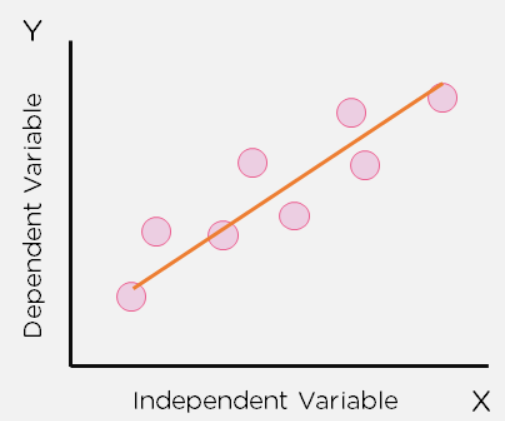
\includegraphics{screenshot001.png}
	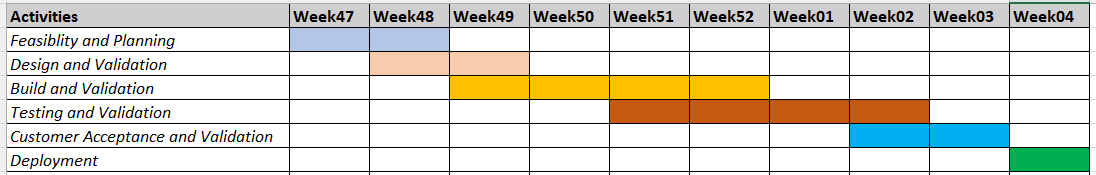
\includegraphics[width=1.2\linewidth]{images/milestone.png}
	\caption{Scheduled Milestone}
\end{figure} 

\section{Risk involved in the Project}
\label{sec:risks}
This document is a model and instructions for \LaTeX.
Please observe the conference page limits. Bla bla 

\section{Effort Estimation}
\label{sec:effort}
Calculating Unadjusted Functional Point
\begin{center}
	\begin{tabular}{ | l | l | l | l | l | l | l | p{3cm} |}
		\hline
		Function type & Simple & Average & Complex & Considered For Project & Count &Total \\ \hline
		External Inputs & 3 & 4 & 5 & 3 & 2 & 6 \\ \hline
		External Output & 4 & 5 & 7 & 5 & 2 & 10 \\ \hline
		External Inquiries  & 3 & 4 & 6 & 5 & 3 & 12 \\ \hline
		Internal Logical Files & 7 & 10 & 15 & 10 & 3 & 30 \\ \hline
		External Interface Files  & 5 & 7 & 10 & 5 & 0 & 0 \\ \hline
		   &   &   &   &   &   & 58 \\ \hline
	\end{tabular}
\end{center}
\textbf{UFP = 58}

\begin{center}
	\begin{tabular}{ | l | l | l | p{3cm} |}
		\hline
		Sr. No & Characteristics & $(0-5)$ \\ \hline
		1 & Data communications & 3  \\ \hline
		2 & Distributed data processing  & 0  \\ \hline
		3 & Performance & 3  \\ \hline
		4 & Heavily used configuration & 0  \\ \hline
		5 & Transaction rate & 5  \\ \hline
		6 & On-Line data entry & 0  \\ \hline
		7 & End-user efficiency & 0  \\ \hline
		8 & On-Line update  & 0  \\ \hline
		9 & Complex processing  & 5  \\ \hline
		10 & Reusability & 2  \\ \hline
		11 & Installation ease & 2  \\ \hline
		12 & Operational ease & 2  \\ \hline
		13 & Facilitate change  & 3  \\ \hline
		14 & Multiple sites  & 0  \\ \hline
		  &   & 25  \\ \hline
	\end{tabular}
\end{center}

 CAF = $0.65+ (0.01 * $∑Fi$)$ \\


CAF = $0.65+ (0.01 * 25) = 0.9$ \\



FPC = $UFP * CAF$
=$58*0.9 = 52.2 ~ 52$. \newpage

\section{Data Flow Diagram}
\label{sec:data-flow}
\begin{figure}
	\centering
	%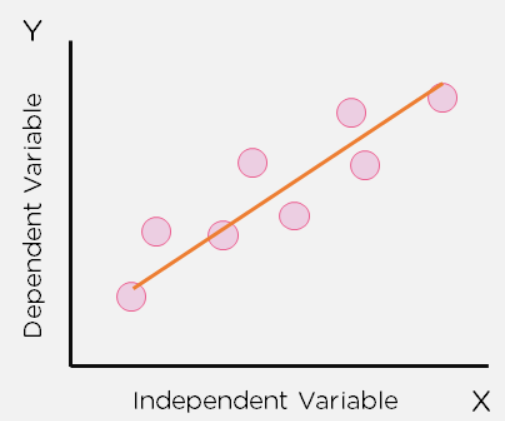
\includegraphics{screenshot001.png}
	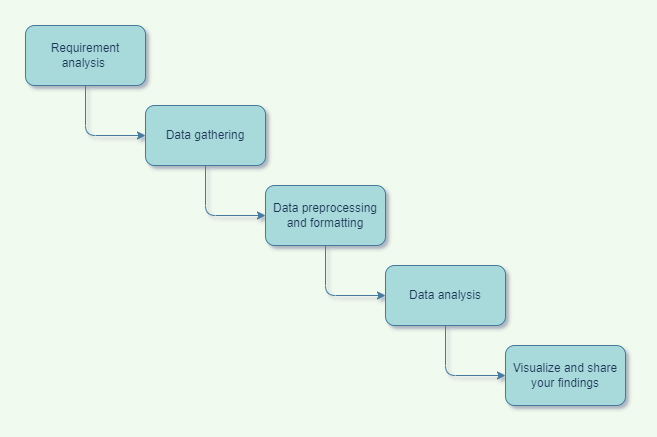
\includegraphics[width=1.2\linewidth]{images/DFD.drawio.png}
	\caption{Data Flow Diagram}
\end{figure}  \newpage

\section{Control Flow Diagram}
\label{sec:control-flow}
\begin{figure}
	\centering
	%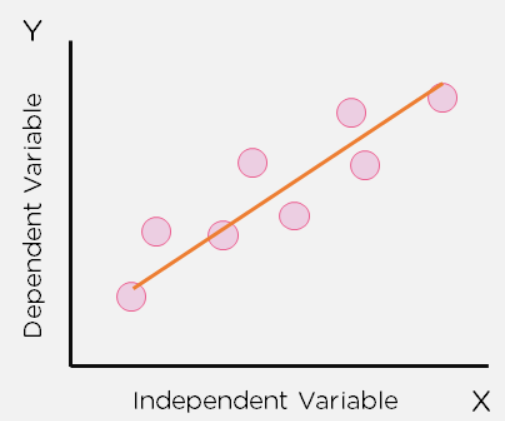
\includegraphics{screenshot001.png}
	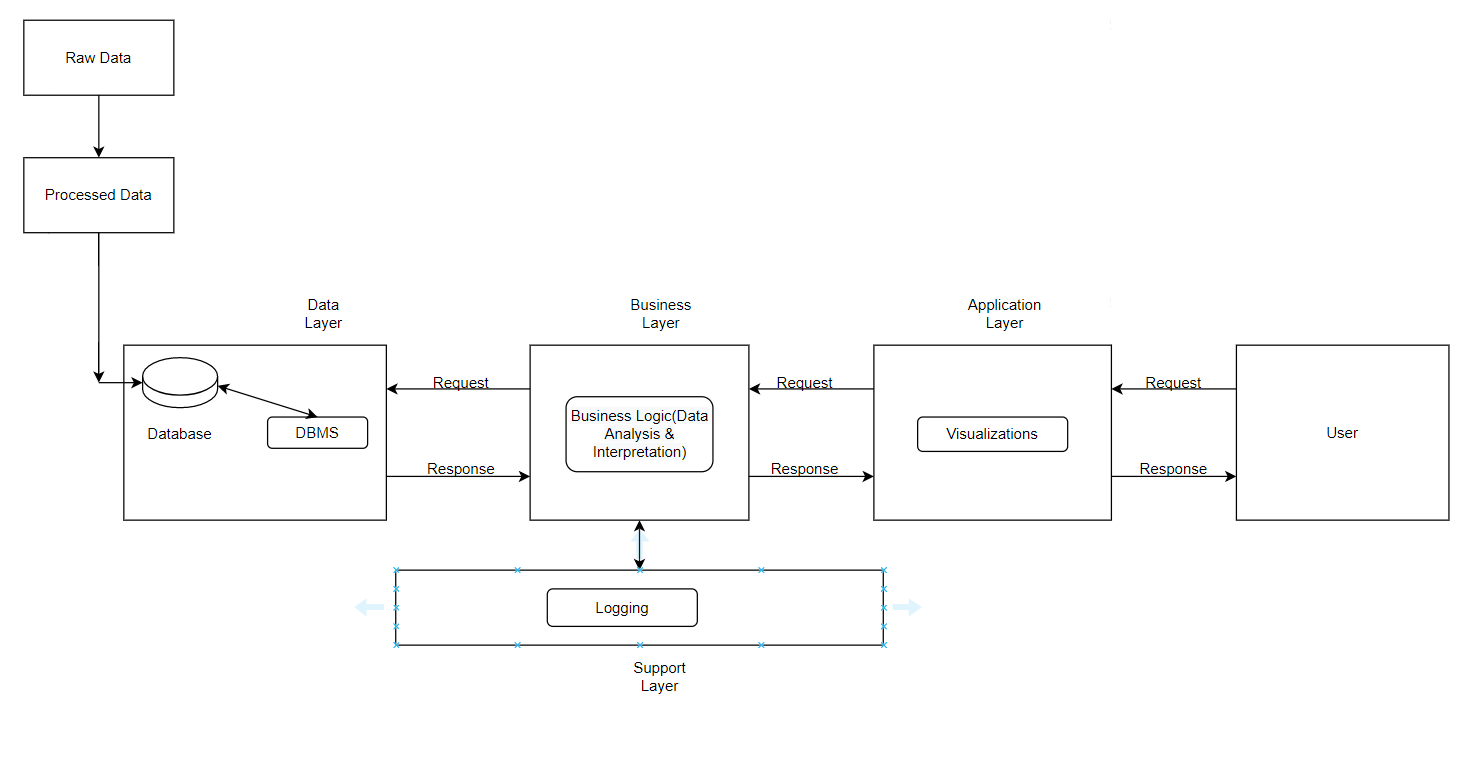
\includegraphics[width=1.2\linewidth]{images/Control Flow.png}
	\caption{Control Flow Diagram}
\end{figure}  \newpage


\section{Use Case Diagram}
\label{sec:use-case-dia}
\begin{figure}
	\centering
	%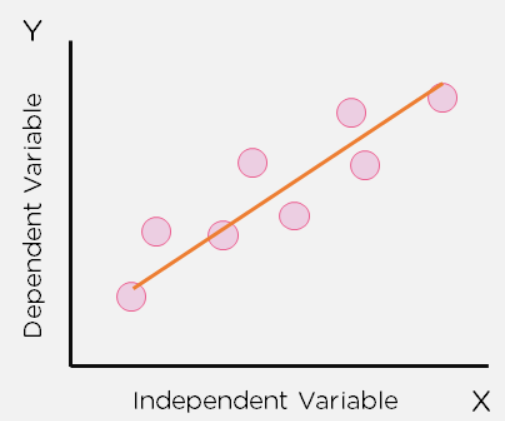
\includegraphics{screenshot001.png}
	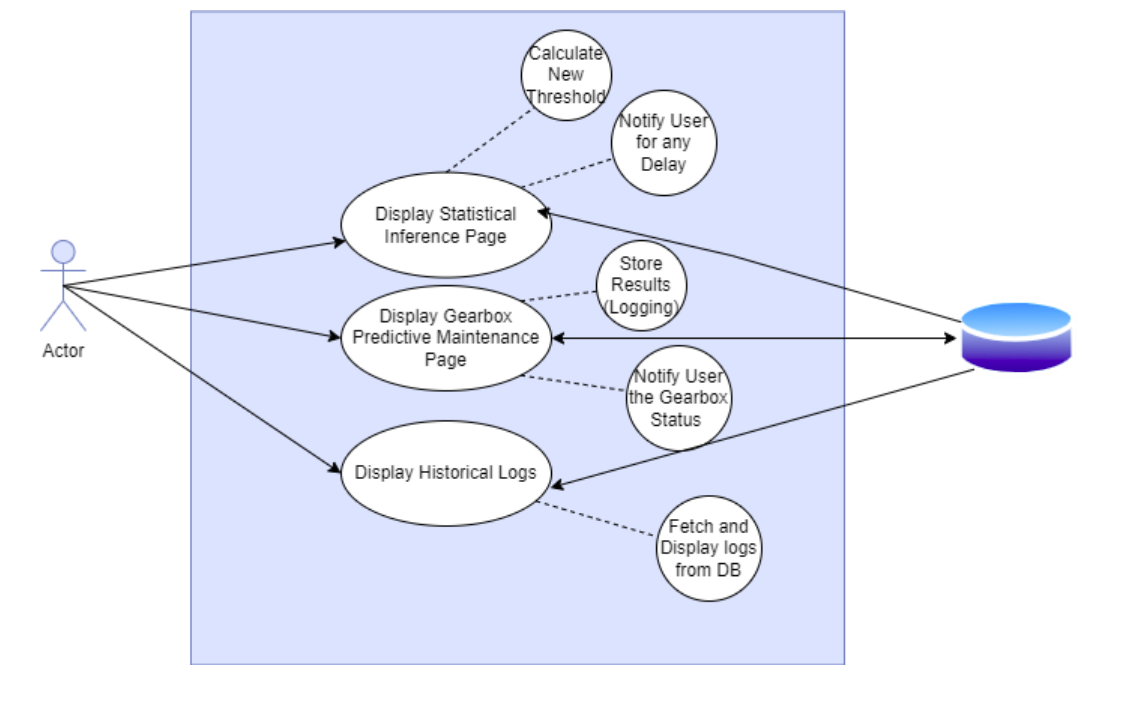
\includegraphics[width=1.2\linewidth]{images/use-case-diagram.png}
	\caption{Use Case Diagram}
\end{figure}  \newpage


\section{Sequence Diagram}

\label{sec:seq-dia}
\begin{figure}
	\centering
	%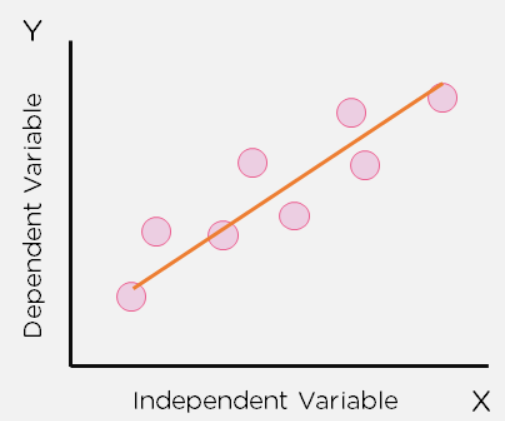
\includegraphics{screenshot001.png}
	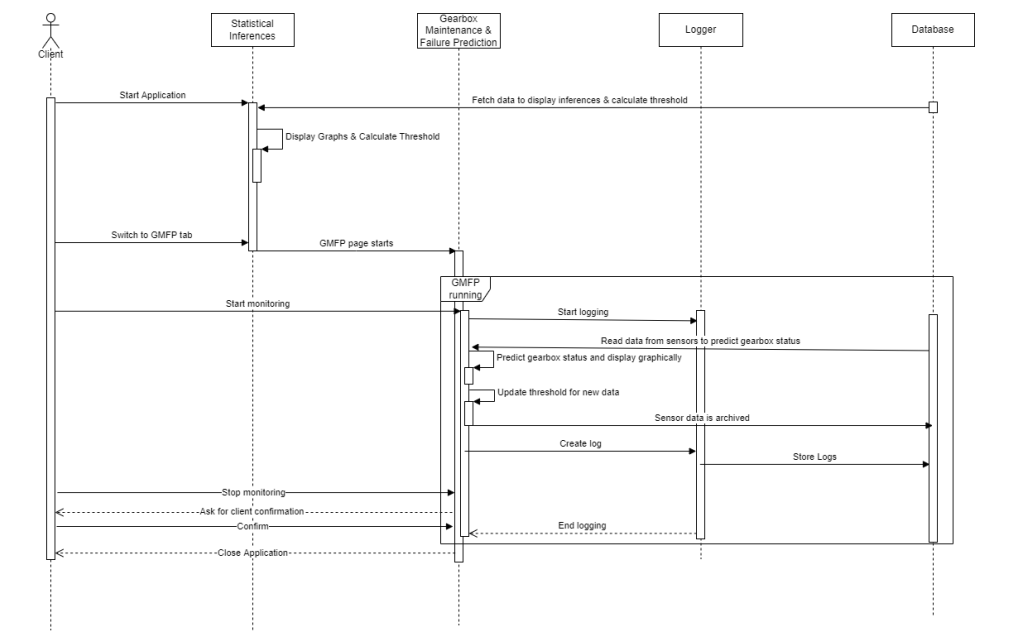
\includegraphics[width=1.2\linewidth]{images/sequence-diagram.png}
	\caption{Sequence Diagram}
\end{figure}  \newpage

\section{System Architecture}
\label{sec:architecture}
\begin{figure}
	\centering
	%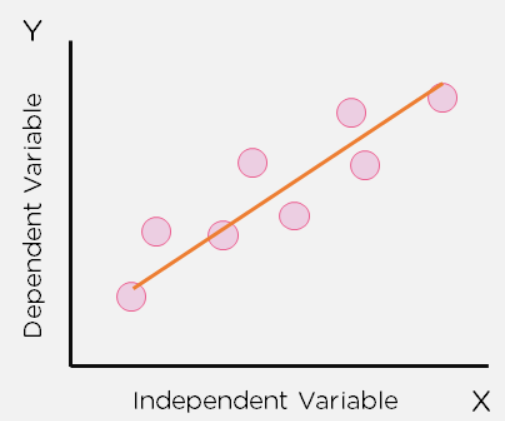
\includegraphics{screenshot001.png}
	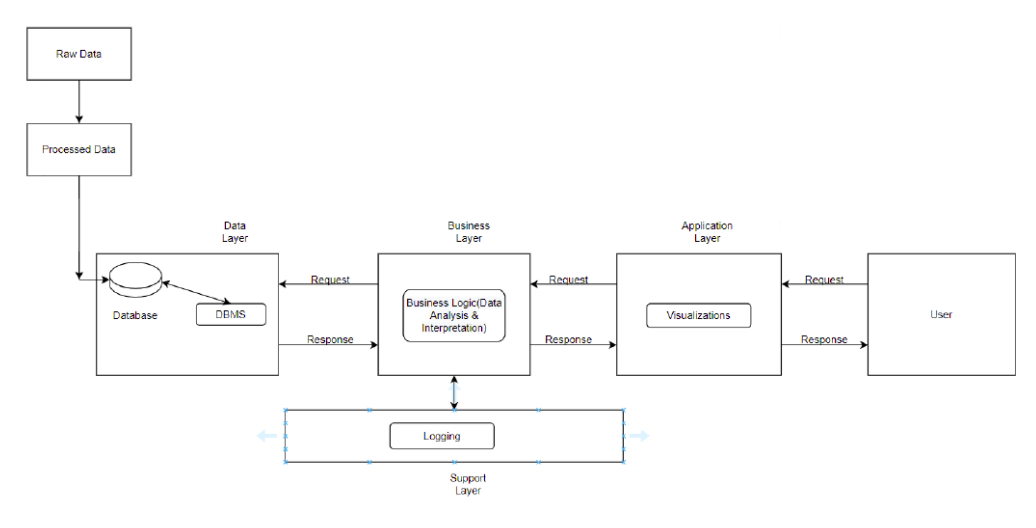
\includegraphics[width=1.2\linewidth]{images/system-architecture.png}
	\caption{Use Case Diagram}
\end{figure}  \newpage

\section{Hazard Analysis}
\label{sec:hazard}
\begin{figure}
	\centering
	%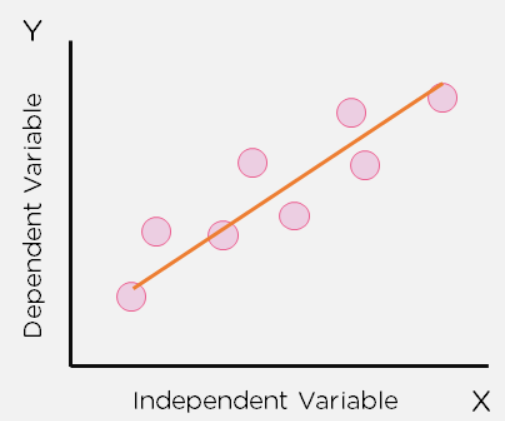
\includegraphics{screenshot001.png}
	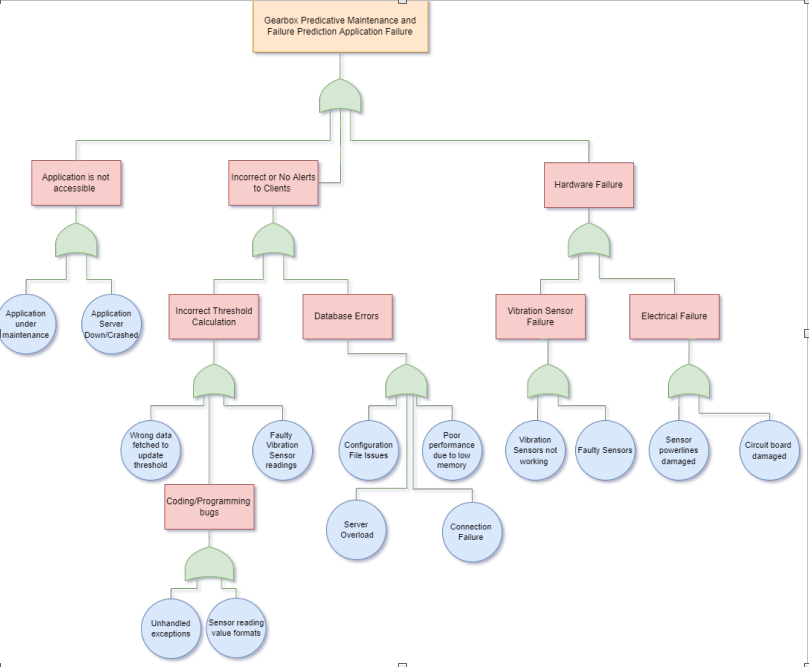
\includegraphics[width=1.2\linewidth]{images/hazard-analysis.png}
	\caption{Use Case Diagram}
\end{figure}  \newpage

\section{Safety Plan}
\label{sec:safety}
The safety plan was created following a thorough examination of the system's hazard analysis results when it is subjected to specific environmental and technical conditions. We incorporated several safety mechanisms that were considered safety constraints within the system if the system failed, because a hazard describes a system’s state that should not occur for safety reasons.  We conducted a preliminary hazard analysis to identify probable hazards and their contributing flaws in a systematic manner. We then chose which flaws to fix and how to mitigate them after discussing with each other. The mitigations were outlined as mandatory safety measures for the system.\\

\subsection{SID: 1}		
\textbf{Hazard Category:} Application is not accessible
\textbf{Hazard:}
\begin{enumerate}
	\item Application under maintenance.
	\item Application server down/crashed
\end{enumerate}
\textbf{Root Cause:}
\begin{enumerate}
	\item Scheduled or planned maintenance
	\item Issues at the client side such as file system corruption
\end{enumerate}
\textbf{Risks:} If the application is unavailable for a considerable amount of time, the data coming from vibration sensors will be lost thus resulting the low reliability. The user will not be able to actively see the status of the gearbox.\\
\textbf{Safety Plan:}
\begin{enumerate}
	\item Notify the user in prior about the downtime due to scheduled maintenance. Once the maintenance is over, the application shall publish the updated status of the gearbox using the data logged during downtime.
	\item While the system is inaccessible, the data coming from the vibration sensors will be directly persisted until it is used to update the threshold. The user will also be provided with certain troubleshooting tips in the user manual. Once the system is available again, the application shall publish the updated status of the gearbox using the data logged during downtime.
\end{enumerate}

\subsection{SID: 2}		
\textbf{Hazard Category:} Incorrect threshold calculation
\textbf{Hazard:}
\begin{enumerate}
	\item Wrong data fetched to update threshold
	\item Faulty vibration sensor readings (Out of scope)
\end{enumerate}
\textbf{Root Cause:}
\begin{enumerate}
	\item Improper transaction management of inconsistent data handling
	\item Wear and tear of vibration sensors
\end{enumerate}
\textbf{Risks:} Inaccurate gearbox status predictions due to incorrect threshold updates\\
\textbf{Safety Plan:}
\begin{enumerate}
	\item Ensure data archival during downtime and orderly transaction execution to update the threshold
	\item Ensure regular maintenance checks of vibration sensors
\end{enumerate}

\subsection{SID: 3}		
\textbf{Hazard Category:} Coding or Programming bugs
\textbf{Hazard:}
\begin{enumerate}
	\item Unhandled Exceptions
	\item Sensor reading value formats
\end{enumerate}
\textbf{Root Cause:}
\begin{enumerate}
	\item Code smells
	\item Conversion between different units of vibration
\end{enumerate}
\textbf{Risks:} 
 \begin{enumerate}
 	\item Application crashes
 	\item Incorrect gearbox status predictions due to incorrect threshold updates
 \end{enumerate}
 
\textbf{Safety Plan:}
\begin{enumerate}
	\item Ensure proper coding guidelines is followed during development and testing
	\item Ensure conversion between different units of vibration is implemented during development phase.
\end{enumerate}

\subsection{SID: 4}		
\textbf{Hazard Category:} Database errors
\textbf{Hazard:}
\begin{enumerate}
	\item Configuration file issues
	\item Poor performance due to low memory
	\item Server overload
	\item Connection failure
\end{enumerate}
\textbf{Root Cause:}
\begin{enumerate}
	\item Improper database deployment
	\item Hardware issues or deadlocks arising due to improper transaction management
	\item Hardware issues or server crashes
\end{enumerate}
\textbf{Risks:} Unavailability of the database might result in loss of data coming from the vibration sensors thus affecting the reliability of the system and incorrect predictions of gearbox status\\
\textbf{Safety Plan:}
\begin{enumerate}
	\item Ensure database is deployed properly
	\item Ensure orderly execution of optimized queries to avoid deadlocks and scheduled maintenance checks should be carried out to ensure proper functioning of the database
	\item Scheduled maintenance checks should be carried out to ensure proper functioning of the database
\end{enumerate}

\subsection{SID: 5}		
\textbf{Hazard Category:} Vibration sensor failure (Out of scope)
\textbf{Hazard:}
\begin{enumerate}
	\item Vibration sensor not working
	\item Faulty sensors
\end{enumerate}
\textbf{Root Cause:}
\begin{enumerate}
	\item Wear and tear
	\item Sensor malfunction
\end{enumerate}
\textbf{Risks:}  Data from one or more sensors will not be logged and thus will result in incorrect gearbox status prediction\\
\textbf{Safety Plan:}
User should be notified if the system is not receiving data from all 4 vibration sensors. The application should not predict gearbox status if at least 1 of the sensors are not working 

\subsection{SID: 5}		
\textbf{Hazard Category:} Electrical failures (Out of scope)
\textbf{Hazard:} Circuit board damaged
\begin{enumerate}
	\item Sensor powerline damaged
	\item Circuit board damaged
\end{enumerate}
\textbf{Root Cause:}
Wear and tear \\
\textbf{Risks:} Data from one or more sensors will not be logged and thus will result in incorrect gearbox status prediction\\
\textbf{Safety Plan:}
User should be notified if the system is not receiving data from all 4 vibration sensors. The application should not predict gearbox status if at least 1 of the sensors are not working.

\section{Question 2}
\label{sec:question}
New technology is causing fundamental changes in the etiology of accidents, necessitating adjustments in the explanatory processes now in use. The most effective models will go beyond assigning guilt and instead assist engineers in learning as much as possible about all of the elements at play, including social and organizational structures. Hazard analysis is essential for ensuring the safety of smart systems that are often controlled by software. Systems-Theoretic Mischance Modelling and Processes (STAMP) has been utilized in different zones to obtain more causal components amid risk examination as a novel causality model. However, the use of STAMP to date has been random, with no formal mechanism in place to efficiently study system threats, and the quality of the analysis results cannot be assured. Additionally, the time element has received less attention in STAMP-based analysis as a key source of risks. This work proposes a systematic technique for hazard analysis based on STAMP in order to overcome these drawbacks. And the Hazardous Control Action Tree (HCAT) is offered as a model and analytical tool for all circumstances that should be addressed in hazard analysis. 


Leveson published Systems-Theoretic Accident Modeling and Processes (STAMP) to capture a broader variety of causative elements than event-chain models and increase the efficacy of software hazard assessments. The STAMP views the mishaps as the result of a lack of control or enforcement of safety limits during the system's development, design, and operation. And, based on STAMP, the System Theoretic Process Analysis (STPA) approach is created to identify the Hazardous Control Action (HCA) as the causes in the hazard analysis, which can violate safety-related constraints and contribute to system hazard. STPA's application, on the other hand, is ad hoc and lacks rigid processes, necessitating greater work, time, and associated deep expertise in the STPA process. 


Although certain support tools, such as SARRA, have been given to aid with the STPA hazard analysis, these tools focus on preserving the consistency or traceability of the data rather than providing a systematic technique to detect the HCAs in the STPA process. The expanded STPA techniques with context table were presented by Thomas and Asim for incorporating all potential environmental factors in the HCA identification of STPA, but these methods do not focus on temporal conditions, and the analysis process still relies on the analysts.


\textbf{Why do we need something new?}
The current problem is that, our tools are 40 to 65 years old. But out technology is very different today. FMEA was introduced between the year 1945-1950. FTA, HAZOP and ETA came in the year 1960-1970. In the late 1970’s people started using computers in control which gave rise to exponential increase in complexity, lots of new technology, new ways of doing things and changes in the way humans work.


Accident models are used to investigate and analyse accidents, as well as to prevent future ones and to determine whether systems are safe to use (risk assessment). They impose patterns on accidents in accident investigations, influencing both the data collected and the elements identified as responsible. They also serve as the foundation for all hazard analysis and risk assessment methods. They may operate as a filter and bias toward evaluating only particular occurrences and conditions, or they may broaden activities by demanding examination of aspects that are normally overlooked, because they alter the factors considered in any of these activities.


Most accident models consider accidents to be the outcome of a series of events. For losses induced by physical component failures and for relatively simple systems, such models function effectively. However, since WWII, the types of systems we've attempted to develop, as well as the context in which they've been built, have shifted. These changes, are pushing the limitations of current accident models and safety engineering procedures, necessitating new approaches.



The changes include-
\begin{itemize}
	\item Increasing technological changes: Technology is evolving at a quicker rate than engineering strategies to deal with it are being developed. When outdated technology are replaced with new ones, lessons accumulated through ages about designing to prevent accidents may be forgotten or rendered worthless.
	\item Variants of Hazards: The most prevalent accident models are founded on the premise that accidents are caused by an uncontrolled and unwanted release of energy or an interruption in the usual flow of energy. Our growing reliance on information systems, however, raises the risk of data loss or incorrect data, which might result in unacceptably large physical, scientific, or financial losses.
	\item Decrease in Single-accident tolerance: As the cost and potential destructiveness of the systems we design rises, so do the losses resulting from accidents. Our new scientific and technological discoveries have not only created new or increased hazards (such as radiation exposure and chemical pollution), but they have also provided the means to harm an increasing number of people as the scale of our systems grows, as well as to negatively impact future generations through pollution and genetic damage. In an age when a spacecraft, for example, might take ten years and cost a billion dollars to develop, financial losses and wasted opportunities for scientific advancement are on the rise. Accident lessons must be augmented with a greater emphasis on preventing the first one.
	\item Changing Nature of Accidents: While digital technology has ushered in a quiet revolution in most sectors of engineering, methodologies in system engineering and system safety engineering have lagged behind. New "failure modes" introduced by digital systems are altering the character of accidents.
	\item Changing public and regulatory awareness of safety: The duty for safety is moving from the individual to the government in our increasingly complicated and interconnected society framework. Individuals no longer have control over the hazards they face, and they are asking that the government take a stronger role in regulating behavior through laws and other types of supervision and regulation. As firms face rising time-to-market and financial challenges, the government will be forced to step in to offer the protection that the public expects. The alternative is for people and groups to appeal to the courts for protection, which might have even worse consequences, such as restricting innovation unnecessarily due to fear of legal action.
	\item ncrease in complexity and coupling: The majority of the elements of complexity, particularly interactive complexity, are rising in the systems we are constructing. We're creating systems with possible interactions between components that can't be completely planned, understood, predicted, or avoided. Some systems are so complicated that they are beyond the comprehension of all but a few specialists, and even they have only a partial knowledge of their possible behavior. Software has helped us implement more integrated, multi-loop control in systems with a large number of dynamically interacting components, where tight coupling allows disruptions or dysfunctional interactions in one part of the system to have far-reaching rippling effects.
	\item Complexity in relationship between Humans and Automation: Humans are increasingly sharing system control with automation and rising into higher-level decision-making roles, with automation carrying out the choices. These changes are leading to various new types of human errors.\\
These developments are putting our accident models, as well as the accident prevention and risk assessment methodologies that are based on them, to the test. There is a need for new paradigms.
	
\end{itemize}


\textbf{An Accident Model Based on Systems Theory}
Systems-Theoretic Accident Model and Processes (STAMP) is a new conception of safety in which accidents occur when external disturbances, component failures, or dysfunctional interactions among system components are not adequately handled by the control system. The hypothesis underlying STAMP is that system theory is a useful way to analyze accidents. In this framework, understanding why an accident occurred requires determining why the control structure was ineffective. Safety then can be viewed as a control problem, and safety is managed by a control structure embedded in an adaptive socio-technical system. A control structure is designed to enforce constraints on system development and system operation that result in safe behavior.



In STAMP, systems are viewed as interrelated components that are kept in a state of dynamic equilibrium by feedback loops of information and control. The original design must not only enforce appropriate constraints on behavior to ensure safe operation, but the system must continue to operate safely as changes occur. Safety management is no longer simply about preventing component failure events. Instead, it is defined as a continuous control task to impose the constraints necessary to limit system behavior to safe changes and adaptations. Accidents can be understood in terms of why the controls that were in place did not prevent or detect mal-adaptive changes.



In STAMP, accidents are defined in terms of violations of safety constraints, which may result from
\begin{enumerate}
	\item system component failure(s),
	\item environmental disturbances, and
	\item  dysfunctional interactions among components
\end{enumerate}


Constraints, control loops and process models, and degrees of control are the fundamental principles of STAMP. Each of them is now detailed, followed by an accident factor categorization based on the new model and core systems theory ideas.


\textbf{The Central Role of Constraints in System Safety}
Safety is an emergent feature in systems theory that occurs when system components interact with their surroundings. A collection of restrictions (control rules) connected to the behavior of the system components govern or enforce emergent features. Accidents are caused by a lack of suitable interaction restrictions. In STAMP, a constraint, not an event, is the most fundamental idea. Accidents are said to occur as a result of a lack of appropriate system limitations. The system engineer, also known as a system safety engineer, is responsible for identifying the design constraints that must be adhered to in order to maintain safety, as well as ensuring that the system design, which includes not only the physical but also the social and organizational aspects of the system, does so.



\end{document}

